\section{Ejercicio 5}
\subsection{Introducción} \label{sec:intro_ex5}
Un ecualizador es un circuito que implementa conocimientos electrónicos en aplicaciones de audio.
El propósito del mismo es, para ciertas frecuencias audibles determinadas por el diseñador, atenuar o amplificar la señal de entrada, 
conforme se haga variar algún parámetro en el circuito (por ejemplo, una resistencia mediante el uso de un potenciómetro).
Es común que estos circuitos vengan implementados en forma repetitiva, para lograr así tener influencia sobre distintas frecuencias del rango audible.
Comercialmente pueden encontrarse ecualizadores de octavas, que refieren a que el dispositivo en su totalidad cuenta con un ecualizador por cada octava en el rango audible,
formando un total de 10 ecualizadores.



\subsection{Resolución teórica del circuito}
A continuación se realizará una explicación paso a paso del método empleado para la resolución de un circuito que sirve como ecualizador para una frecuencia específica.
Se toma el circuito de la Figura \ref{fig:EQ_module} y se asume comportamiento ideal del operacional.
\begin{figure}[H]
    \centering
    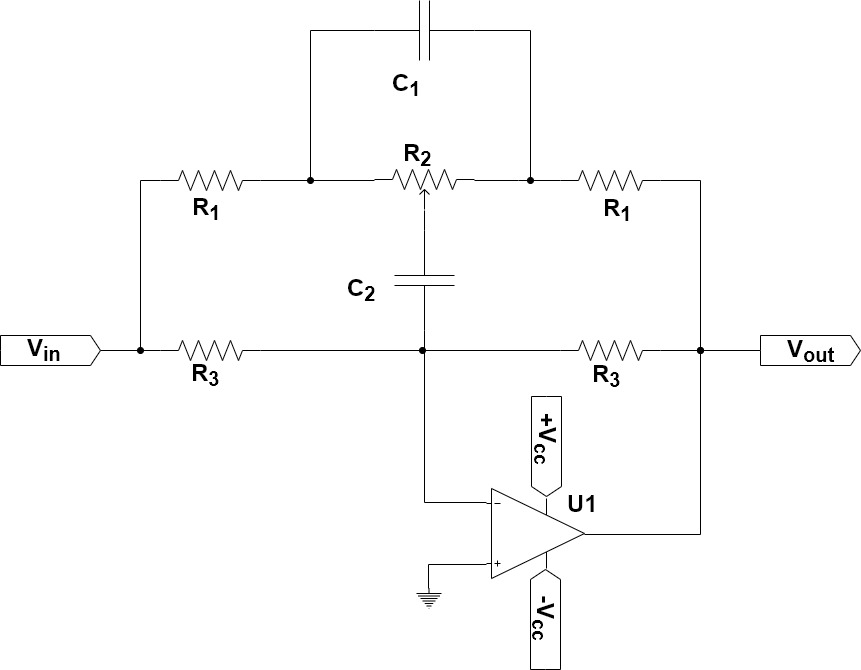
\includegraphics[width=0.6\textwidth]{../EJ5/latex_resources/EQ_module}
    \caption{Circuito ecualizador.}
    \label{fig:EQ_module}
\end{figure}

Se observa que las resistencias $R_2'$, $R_2''$ y $C_1$ se encuentran en configuración $\pi$, y mediante transformaciones de Kennelly se obtienen las impedancias 
de la ecuación \ref{eq:ej5_z1}.
\begin{figure}[H]
    \centering
    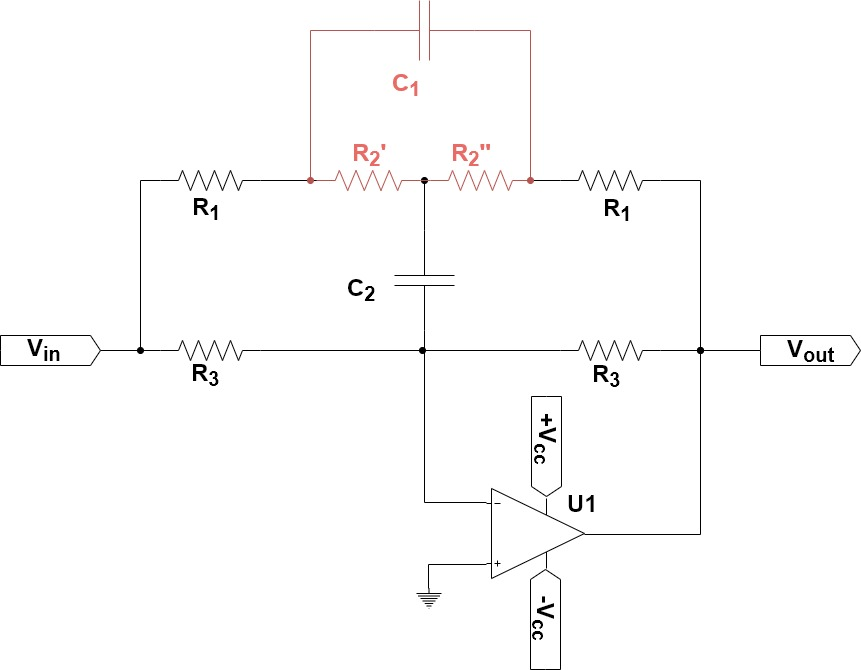
\includegraphics[width=0.6\textwidth]{../EJ5/latex_resources/Z1_2_and_3}
    \caption{Cálculo intermedio.}
    \label{fig:Z123}
\end{figure}

\begin{align}
    &Z_1 = \frac{R_2' \cdot \frac{1}{s \cdot C_1}}{R_2' + \frac{1}{s \cdot C_1} + R_2''}  \label{eq:ej5_z1} \\
    &Z_2 = \frac{R_2'' \cdot \frac{1}{s \cdot C_1}}{R_2' + \frac{1}{s \cdot C_1} + R_2''}  \label{eq:ej5_z2} \\
    &Z_3 = \frac{R_2'' \cdot R_2'}{R_2' + \frac{1}{s \cdot C_1} + R_2''}  \label{eq:ej5_z3} \\
    &R_2 = R_2' + R_2'' \label{eq:ej5_r2}
\end{align}

El resultado de esta transformación puede verse reflejado en la Figura \ref{fig:Z456}.
Además, en la misma puede notarse que nuevamente los componentes remarcados en rojo pueden ser modificados por impedancias equivalentes, aplicando nuevamente Kenelly, 
esta vez para pasar de una configuración T a una $\pi$.
Las impedancias resultantes son las descriptas por la ecuación \ref{eq:ej5_z4}.
\begin{figure}[H]
    \centering
    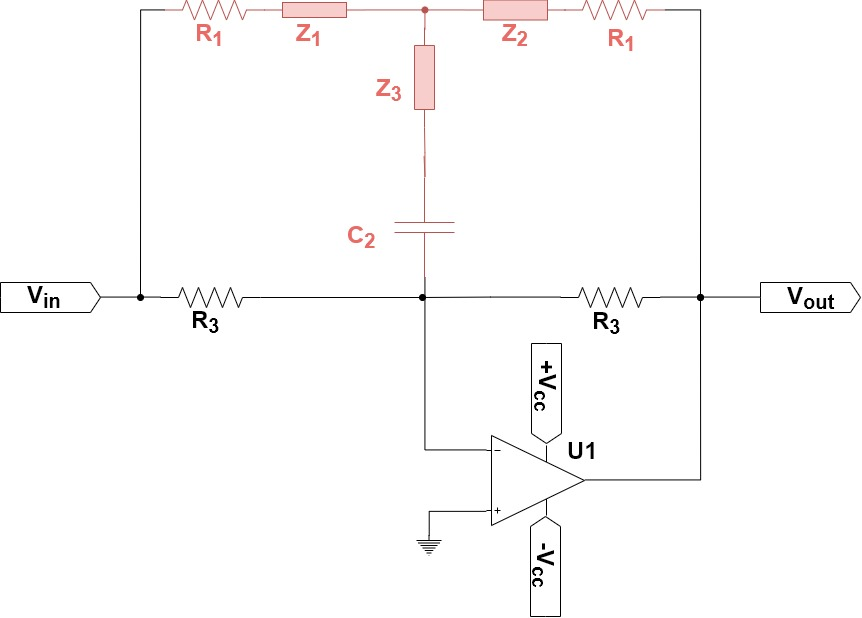
\includegraphics[width=0.6\textwidth]{../EJ5/latex_resources/Z4_5_and_6}
    \caption{Cálculo intermedio.}
    \label{fig:Z456}
\end{figure}

\begin{align}
    &Z_4 = \frac{\left(Z_1 + R_1\right) \cdot \left(Z_2 + R_1\right) + \left(Z_1 + R_1\right) \cdot \left(Z_3 + \frac{1}{s \cdot C_2}\right) + \left(Z_3 + \frac{1}{s \cdot C_2}\right) \cdot \left(Z_2 + R_1\right)}{Z_2 + R_1}  \label{eq:ej5_z4} \\
    &Z_5 = \frac{\left(Z_1 + R_1\right) \cdot \left(Z_2 + R_1\right) + \left(Z_1 + R_1\right) \cdot \left(Z_3 + \frac{1}{s \cdot C_2}\right) + \left(Z_3 + \frac{1}{s \cdot C_2}\right) \cdot \left(Z_2 + R_1\right)}{Z_3 + \frac{1}{s \cdot C_2}}  \label{eq:ej5_z5} \\
    &Z_6 = \frac{\left(Z_1 + R_1\right) \cdot \left(Z_2 + R_1\right) + \left(Z_1 + R_1\right) \cdot \left(Z_3 + \frac{1}{s \cdot C_2}\right) + \left(Z_3 + \frac{1}{s \cdot C_2}\right) \cdot \left(Z_2 + R_1\right)}{Z_1 + R_1}  \label{eq:ej5_z6}
\end{align}

El circuito resultante es el de la Figura \ref{fig:Z78}, al cual le cabe una última modificación para arribar al final de la resolución del circuito.
Se toman las impedancias equivalentes de los paralelos resaltados en rojo, y se obtienen así un nuevo par de impedancias $Z_7$ y $Z_8$.
De la observación del circuito resultante, se obtiene que se trata de un inversor, y que, por lo tanto, la función transferencia está dada por la expresión en \ref{eq:non_inverter_transf_ex5}.
\begin{figure}[H]
    \centering
    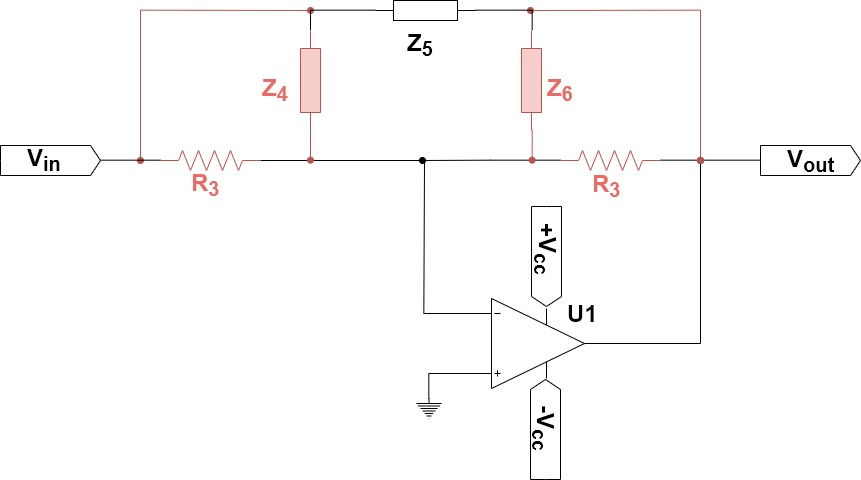
\includegraphics[width=0.6\textwidth]{../EJ5/latex_resources/Z7_and_8}
    \caption{Cálculo intermedio.}
    \label{fig:Z78}
\end{figure}

\begin{align}
    &Z_7 = \frac{R_3 \cdot Z_4}{R_3 + Z_4} \label{eq:ej5_z7} \\
    &Z_8 = \frac{R_3 \cdot Z_6}{R_3 + Z_6} \label{eq:ej5_z8}
\end{align}

\begin{align}
    &\frac{v_{out}}{v_{in}} = - \frac{Z_8}{Z_7} \label{eq:non_inverter_transf_ex5}
\end{align}

Reemplazando los valores de las impedancias por sus equivalentes en términos de $R_1$, $R_2$, $R_3$, $C_1$ y $C_2$, se llega a la siguiente expresión de la transferencia del circuito.
\begin{ssmall}
\begin{adjustwidth*}{-1.3cm}{}
    \begin{align}
        &\frac{v_{out}}{v_{in}} = - \frac{C_1 \cdot C_2 \cdot R_1 \cdot \left(R_1 \cdot R_2 - 2 \cdot R_2'^2 + 2 \cdot R_2 \cdot R_2' + R_2 \cdot R_3\right) \cdot s^2 +
                                        \left(2 \cdot C_1 \cdot R_1 \cdot R_2 + C_2 \left(R_1^2 + R_1 \cdot \left(R_2 + R_3\right) - \left(R_2' + R_3\right) \cdot \left(R_2' - R_2\right)\right)\right) \cdot s +
                                        2 \cdot R_1 + R_2}
                                        {C_1 \cdot C_2 \cdot R_1 \cdot \left(R_1 \cdot R_2 - 2 \cdot R_2'^2 + 2 \cdot R_2 \cdot R_2' + R_2 \cdot R_3\right) \cdot s^2 +
                                        \left(2 \cdot C_1 \cdot R_1 \cdot R_2 + C_2 \left(R_1^2 + R_1 \cdot \left(R_2 + R_3\right) - R_2' \cdot \left(R_2' - R_2 - R_3\right)\right)\right) \cdot s +
                                        2 \cdot R_1 + R_2} \label{eq:ej5_complete_transference}
    \end{align}
\end{adjustwidth*}
\end{ssmall}

La aplicación de las relaciones en \ref{eq:EQ_relations_ex5} llevan de la ecuación \ref{eq:ej5_complete_transference} a la \ref{eq:ej5_approx_transference}, 
siendo esta última la que será utilizada como transferencia del sistema.
\begin{align}
    &R_3 >> R_1 \label{eq:EQ_relations_ex5}\\
    &R_3 = 10 \cdot R_2 \\
    &C_1 = 10 \cdot C_2
\end{align}

\begin{align}
    &\frac{v_{out}}{v_{in}} = - \frac{\frac{20 \cdot C_2^2 \cdot R_1 \cdot \left(R_2 \cdot R_2' + 5 \cdot R_2^2 - R_2'^2\right)}{2 \cdot R_1 + R_2} \cdot s^2 +
                                        \frac{C_2 \cdot \left(30 \cdot R_1 \cdot R_2 + \left(R_2 - R_2'\right) \cdot \left(R_2' + 10 \cdot R_2\right)\right)}{2 \cdot R_1 + R_2} \cdot s +
                                        1}
                                        {\frac{20 \cdot C_2^2 \cdot R_1 \cdot \left(R_2 \cdot R_2' + 5 \cdot R_2^2 - R_2'^2\right)}{2 \cdot R_1 + R_2} \cdot s^2 +
                                        \frac{C_2 \cdot \left(31 \cdot R_1 \cdot R_2 + R_2' \cdot \left(11 \cdot R_2 - R_2'\right)\right)}{2 \cdot R_1 + R_2} \cdot s +
                                        1} \label{eq:ej5_approx_transference}
\end{align}

De esta última expresión se obtiene que la frecuencia de corte para el filtro de segundo órden viene dada por la ecuación \ref{eq:ej5_notch_frequency}.
\begin{align}
    &f_0 = \frac{\sqrt{\frac{5 \cdot \left(2 \cdot R_1 + R_2\right)}{R_1 \cdot \left(5 \cdot R_2^2 + R_2 \cdot R_2' - R_2'^2\right)}}}{20 \pi \cdot C_2}
    \label{eq:ej5_notch_frequency}
\end{align}

Un estudio de la frecuencia de corte en los casos límite, es decir con $R_2' = 0$ y $R_2' = R_2$, que representan los dos extremos del potenciómetro, 
demuestra que la misma es fija y del valor expresado en la siguiente ecuación:
\begin{align}
    &f_0 = \frac{\sqrt{2 + \frac{R_2}{R_1}}}{20 \pi \cdot R_2 \cdot C_2}
    \label{eq:ej5_notch_frequency_limit_cases}
\end{align}

Por otro lado, si se observa la ganancia en dicha frecuencia de corte, se llega a que la misma está dada por la siguiente expresión:
\begin{align}
    &A_0 = - \frac{30 \cdot R_1 \cdot R_2 + \left(R_2 - R_2'\right) \cdot \left(10 \cdot R_2 + R_2'\right)}{31 \cdot R_1 \cdot R_2 + R_2' \cdot \left(11 \cdot R_2 - R_2'\right)}
    \label{eq:ej5_system_gain}
\end{align}

La misma puede también ser estudiada en sus casos límite (nuevamente, con $R_2' = 0$ y $R_2' = R_2$), y el resultado que se obtiene ahora es distinto e interesante.
En primer lugar, para $R_2' = 0$:
\begin{align}
    &A_0 = - \frac{30 \cdot R_1 + 10 \cdot R_2}{31 \cdot R_1} \approx \frac{3 \cdot R_1 + R_2}{3 \cdot R_1}
    \label{eq:ej5_system_gain_for_R2'_0}
\end{align}

Y luego para $R_2' = R_2$:
\begin{align}
    &A_0 = - \frac{30 \cdot R_1}{31 \cdot R_1 + 10 \cdot R_2} \approx \frac{3 \cdot R_1}{3 \cdot R_1 + R_2}
    \label{eq:ej5_system_gain_for_R2'_R2}
\end{align}

Ha de observarse que la variación de la resistencia en el potenciómetro genera una inversión en la ganancia, es decir, dados ciertos valores de $R_1$ y $R_2$, 
el circuito amplifica y atenúa en la misma proporción, con el potenciómetro volcado hacia $R_2'$ o $R_2''$, respectivamente.
Además, es relevante remarcar que este circuito tendrá ganancia cercana a 0 dB en frecuencias alejadas la de corte.
Qué se considera como "alejadas" dependerá de la selectividad del filtro y, por lo tanto, de parámetros de diseño.



\subsection{Caracterización de polos y ceros}
La caracterización de polos y ceros consiste básicamente en la observación de su posición en el plano complejo, para las distintas posiciones del potenciómetro.
Se realizó un estudio de los mismos para 75 valores distintos de $R_2'$ y $R_2''$, y los resultados son los expuestos en la Figura \ref{fig:poles_and_zeros_diag_ej5}.
\begin{figure}[H]
    \centering
    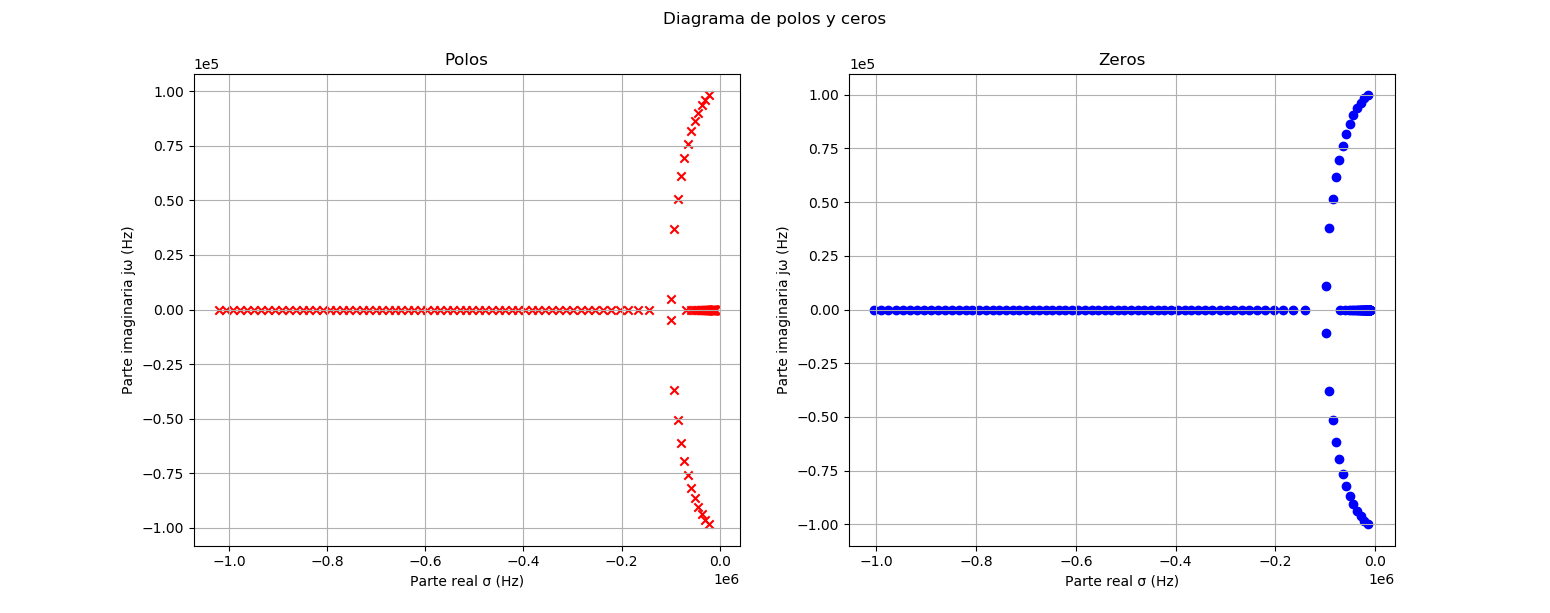
\includegraphics[width=\textwidth]{../EJ5/latex_resources/diagrama_polos_y_ceros}
    \caption{Diagramas de polos y ceros}
    \label{fig:poles_and_zeros_diag_ej5}
\end{figure}

Nótese como, sin importar la variación en las resistencias del potenciómetro, tanto los polos como los ceros se encuentran en el semiplano izquierdo, indicando que el 
circuito es consistentemente estable y de fase mínima.

Ante el cuestionamiento de si el circuito puede convertirse en uno de fase no mínima, mediante la alteración de alguno de los valores de sus componentes, se procede a 
estudiar sus ceros, y se llega a que los mismos son los de la ecuación \ref{eq:ej5_num_roots_simplyfied_system}.
Para simplificar estos cálculos se decidió expresar $R_2' = \epsilon \cdot R_2$ y $R_2'' = (1-\epsilon) \cdot R_2$, con $0 \leq \epsilon \leq 1$
\begin{ssmall}
\begin{align}
    &\frac{-30 \cdot R_1 + R_2 \cdot \epsilon^2 + 9 \cdot R_2 \cdot \epsilon - 10 \cdot R_2 - \sqrt{R_1^2 \cdot \left(160 \cdot \epsilon^2 - 160 \cdot \epsilon + 100\right) + R_1 \cdot R_2 \cdot \left(20 \cdot \epsilon^2 - 620 \cdot \epsilon + 200\right) + R_2^2 \cdot \left(\epsilon^4 + 18 \cdot \epsilon^3 + 61 \cdot \epsilon^2 - 180 \cdot \epsilon + 100\right)}}{40 \cdot C_2 \cdot R_1 \cdot R_2 \cdot (-\epsilon^2 + \epsilon + 5)} \\
    &\frac{-30 \cdot R_1 + R_2 \cdot \epsilon^2 + 9 \cdot R_2 \cdot \epsilon - 10 \cdot R_2 + \sqrt{R_1^2 \cdot \left(160 \cdot \epsilon^2 - 160 \cdot \epsilon + 100\right) + R_1 \cdot R_2 \cdot \left(20 \cdot \epsilon^2 - 620 \cdot \epsilon + 200\right) + R_2^2 \cdot \left(\epsilon^4 + 18 \cdot \epsilon^3 + 61 \cdot \epsilon^2 - 180 \cdot \epsilon + 100\right)}}{40 \cdot C_2 \cdot R_1 \cdot R_2 \cdot (-\epsilon^2 + \epsilon + 5)} 
    \label{eq:ej5_num_roots_simplyfied_system}
\end{align}
\end{ssmall}

%Raíces del numerador de la transferencia completa:
%\begin{ssmall}
%\begin{align}
%    \frac{-R_1^2 - 31 \cdot R_1 \cdot R_2 + R_2^2 \cdot \epsilon^2 + 9 \cdot R_2^2 \cdot \epsilon - 10 \cdot R_2^2 - \sqrt{R_1^4 - 18 \cdot R_1^3 \cdot R_2 + 158 \cdot R_1^2 \cdot R_2^2 \cdot \epsilon^2 - 178 \cdot R_1^2 \cdot R_2^2 \cdot \epsilon + 141 \cdot R_1^2 \cdot R_2^2 + 18 \cdot R_1 \cdot R_2^3 \cdot \epsilon^2 - 638 \cdot R_1 \cdot R_2^3 \cdot \epsilon + 220 \cdot R_1 \cdot R_2^3 + R_2^4 \cdot \epsilon^4 + 18 \cdot R_2^4 \cdot \epsilon^3 + 61 \cdot R_2^4 \cdot \epsilon^2 - 180 \cdot R_2^4 \cdot \epsilon + 100 \cdot R_2^4}}{20 \cdot C_2 \cdot R_1 \cdot R_2 \cdot (R_1 - 2 \cdot R_2 \cdot \epsilon^2 + 2 \cdot R_2 \cdot \epsilon + 10 \cdot R_2} \\
%    \frac{-R_1^2 - 31 \cdot R_1 \cdot R_2 + R_2^2 \cdot \epsilon^2 + 9 \cdot R_2^2 \cdot \epsilon - 10 \cdot R_2^2 + \sqrt{R_1^4 - 18 \cdot R_1^3 \cdot R_2 + 158 \cdot R_1^2 \cdot R_2^2 \cdot \epsilon^2 - 178 \cdot R_1^2 \cdot R_2^2 \cdot \epsilon + 141 \cdot R_1^2 \cdot R_2^2 + 18 \cdot R_1 \cdot R_2^3 \cdot \epsilon^2 - 638 \cdot R_1 \cdot R_2^3 \cdot \epsilon + 220 \cdot R_1 \cdot R_2^3 + R_2^4 \cdot \epsilon^4 + 18 \cdot R_2^4 \cdot \epsilon^3 + 61 \cdot R_2^4 \cdot \epsilon^2 - 180 \cdot R_2^4 \cdot \epsilon + 100 \cdot R_2^4}}{20 \cdot C_2 \cdot R_1 \cdot R_2 \cdot (R_1 - 2 \cdot R_2 \cdot \epsilon^2 + 2 \cdot R_2 \cdot \epsilon + 10 \cdot R_2}
%    \label{eq:ej5_num_root}
%\end{align}
%\end{ssmall}

Dado que el denominador en esta última expresión es positivo, la primer forma propuesta para que los ceros queden con parte real positiva es que se cumpla que la parte no 
afectada por la raíz sea mayor a 0.
\begin{align}
    &-30 \cdot R_1 + R_2 \cdot \epsilon^2 + 9 \cdot \epsilon - 10 \cdot R_2 > 0
    \label{eq:ej5_attempting_changing_zeros_with_real_part}
\end{align}

Operando a partir de esta relación y considerando $\epsilon = 0$ se llega a:
\begin{align}
    &R_1 < -\frac{1}{3} \cdot R_2
    \label{eq:ej5_results_of_attempting_changing_zeros_with_real_part_epsilon_0}
\end{align}

Luego con $\epsilon = 1$:
\begin{align}
    &R_1 < 0
    \label{eq:ej5_results_of_attempting_changing_zeros_with_real_part_epsilon_1}
\end{align}

En ambos casos, puede observarse con facilidad que la condición es absurda.

Se procede luego a intentar que la parte con la raíz sea mayor en módulo a aquella sin, buscando así raíces reales positivas.
\begin{ssmall}
\begin{align}
    \left|-30 \cdot R_1 + R_2 \cdot \epsilon^2 + 9 \cdot \epsilon - 10 \cdot R_2 \right| < \left|\sqrt{R_1^2 \cdot \left(160 \cdot \epsilon^2 - 160 \cdot \epsilon + 100\right) + R_1 \cdot R_2 \cdot \left(20 \cdot \epsilon^2 - 620 \cdot \epsilon + 200\right) + R_2^2 \cdot \left(\epsilon^4 + 18 \cdot \epsilon^3 + 61 \cdot \epsilon^2 - 180 \cdot \epsilon + 100\right)}\right|
    \label{eq:ej5_attempting_changing_zeros_with_root}
\end{align}
\end{ssmall}

Nuevamente se intenta para $\epsilon = 0$:
\begin{align}
    &3 \cdot R_1 + R_2 < R_1 + R_2
    \label{eq:ej5_results_of_attempting_changing_zeros_with_root_epsilon_0}
\end{align}

Y para $\epsilon = 1$:
\begin{align}
    &800 \cdot R_1 < -4 \cdot R_2
    \label{eq:ej5_results_of_attempting_changing_zeros_with_root_epsilon_1}
\end{align}
Y nuevamente el resultado es absurdo. \par
Se llega así a la conclusión de que es imposible hacer que el sistema sea de fase no mínima, únicamente mediante la alteración de sus parámetros.
De ser necesaria esta condición, se propone como solución al problema agregar una segunda etapa al circuito que conste de un pasa todo de segundo orden, con polos en 
donde el ecualizador tiene ceros (en el semiplano izquierdo), que se encarguen de "cancelarlos", y ceros simétricos pero en el semiplano derecho.



\subsection{Diseño de ecualizador de 3 bandas}
Para el diseño de un ecualizador de 3 bandas se utilizan tres circuitos como los vistos previamente, cuyas frecuencias de corte son elegidas bajo un cierto criterio.
Como se dijo en la introducción (\ref{sec:intro_ex5}), lo ideal es contar con un circuito ecualizador por cada una de las octavas audibles.
Las mismas son 31Hz, 63Hz, 125Hz, 250Hz, 500Hz, 1KHz, 2KHz, 4KHz, 8KHz y 16KHz, tomando 1KHz como la central, y a fin de abarcar el rango de forma más equiparada con los 
tres ecualizadores disponibles, se buscó diseñar los mismos para que tengan sus frecuencias de corte en torno a 125Hz, 1KHz y 8KHz.
Utilizando valores comerciales de potenciómetros y resistencias, se llega a las siguientes frecuencias de corte:
Las frecuencias para las 3 bandas, usando \ref{eq:ej5_notch_frequency_limit_cases}:
\begin{align}
    &f_{01} = \frac{\sqrt{2 + \frac{100 K\Omega}{120\Omega}}}{20\pi \cdot 100 K\Omega \cdot 47 nF} = 97.87 Hz \\
    &f_{02} = \frac{\sqrt{2 + \frac{1 K\Omega}{120\Omega}}}{20\pi \cdot 1 K\Omega \cdot 47 nF} = 1.089 KHz \\
    &f_{03} = \frac{\sqrt{2 + \frac{1 K\Omega}{150\Omega}}}{20\pi \cdot 1 K\Omega \cdot 5.6 nF} = 8.367 KHz
\end{align}

El segundo factor a definir es la interconexion de los módulos.
Por un lado, los tres ecualizadores pueden conectarse en paralelo, y luego mezclar las señales de salida mediante el uso de un sumador.
La ventaja que provee esta configuración es una mejor performance en términos del ruido, ya que cada rama tiene únicamente una etapa de amplificación.
Sin embargo, se corre el riesgo de, en algunas frecuencias, sumar señales que no se encuentren en fase entre ellas, y por lo tanto, que la mezcla de las mismas arroje 
resultados inesperados y distorsiones indeseadas. \par
La segunda opción, es conectar las etapas en cascada, lo cual es viable gracias a que los ecualizadores tienen ganancia 0 dB en las frecuencias alejadas de la de corte de 
cada uno. Consecuentemente, si las frecuencias de corte están debidamente espaciadas, la injerencia de una etapa sobre la otra no será significativa.
Al contrario de la primer opción, esta puede presentar mayores problemas en cuanto al ruido, pero no conlleva peligro alguno en lo que respecta a la fase, ya que la misma 
puede ser modificada sin cuidado alguno a que las señales deban ser sumadas, y el oído humano no es capaz de oir cambios en la fase, cumpliéndose a la perfección el 
objetivo de diseño del circuito. \par
Para tomar una decisión al respecto de qué configuración usar, se simularon ambas opciones atenuando en frecuencias bajas y altas, y amplificando las medias, ambos casi en 
el máximo de atenuación y amplificación, respectivamente, para que a la salida se evidencie la independencia (o no, en caso de no funcionar), de las etapas. \par
Los resultados son los expuestos en la Figura \ref{fig:cascade_v_parallel_ex5}, y de la misma se puede derivar la elección de una configuración en cascada de las etapas.
\begin{figure}[H]
    \centering
    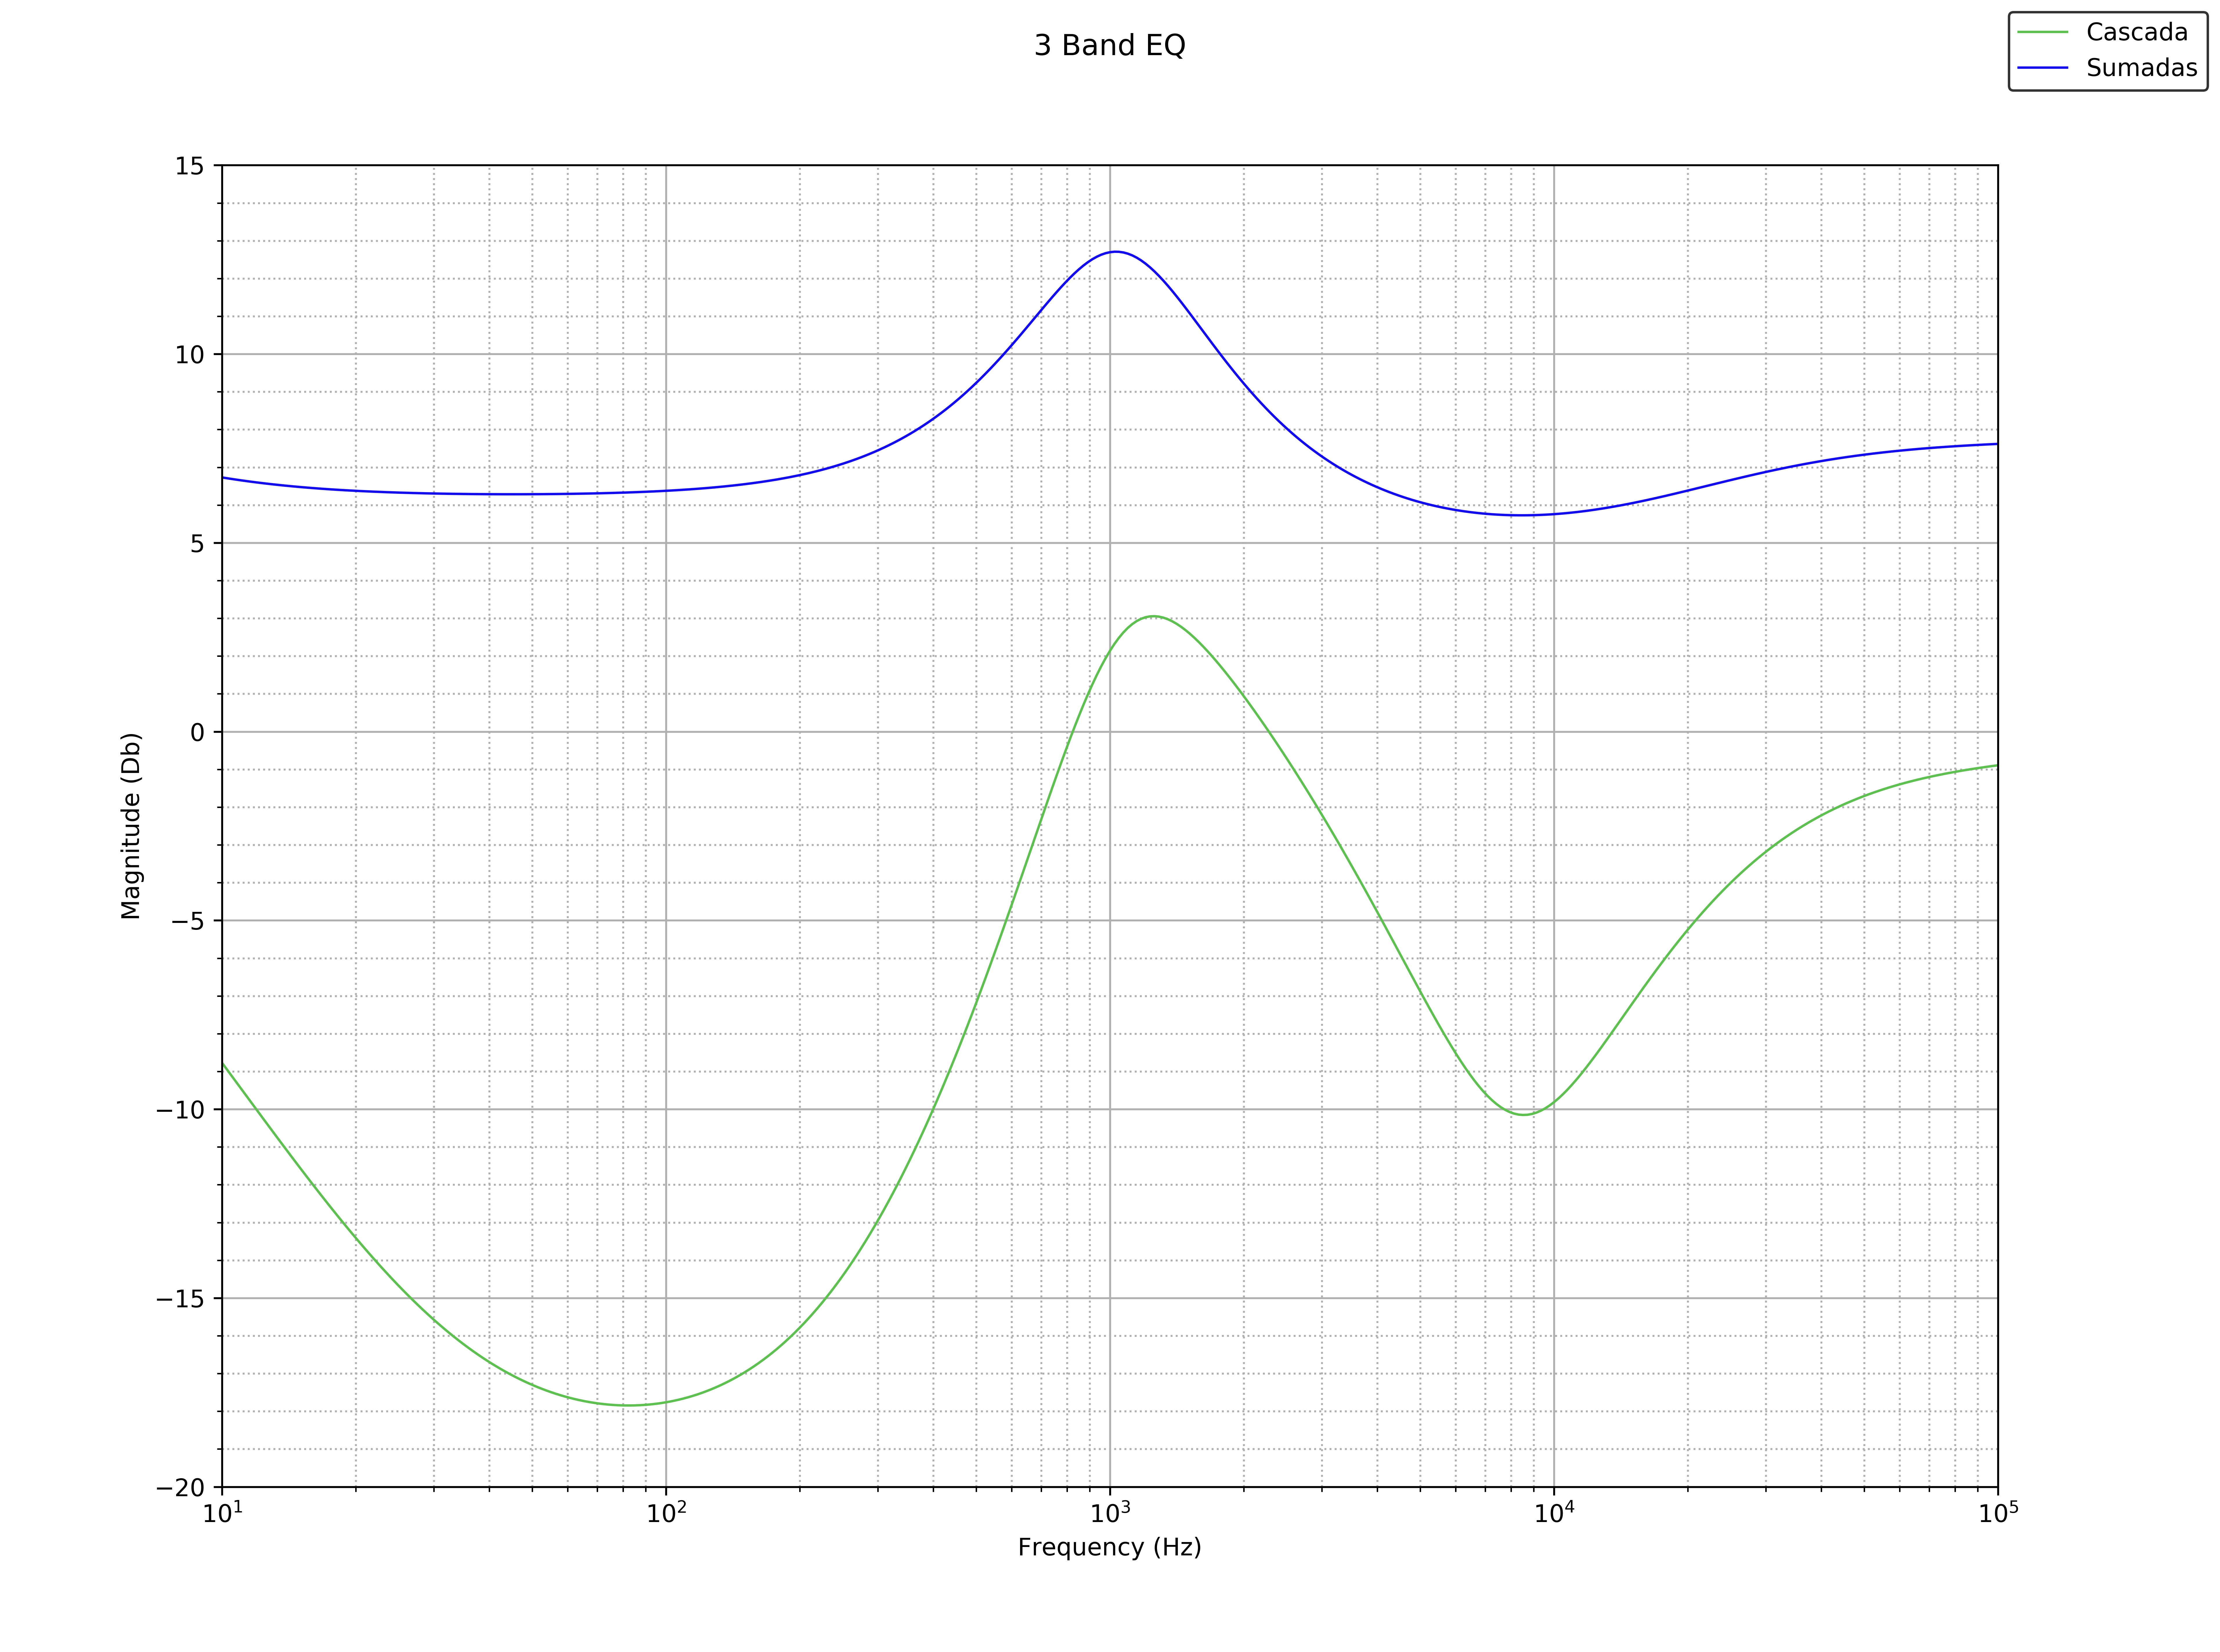
\includegraphics[width=\textwidth]{../EJ5/latex_resources/cascade_v_parallel_comparison}
    \caption{Comparación conexión cascada vs paralelo.}
    \label{fig:cascade_v_parallel_ex5}
\end{figure}

Evidentemente la fase tuvo un papel perjudicial en la suma de las señales en paralelo, ya que el resultado esta lejos de ser el esperado, en el cual debía haber una 
atenuación en frecuencias bajas y altas, y amplificación en las medias.
Se observa en el gráfico que el resultado es una amplificación variable en todas las frecuencias, pero amplificación al fin. \par
Por otro lado, los resultados de la conexión en cascada se asemejan más a lo esperado, ya que en esta configuración sí pueden observarse dos etapas de atenuación y una de 
amplificación, a pesar de que la atenuación no sea simétrica con la amplificación. Se atribuye esta discrepancia con lo esperado a la injerencia de una etapa sobre la 
sucesiva, efecto que es perjudicial al diseño, pero es de todas formas preferible por sobre los resultados obtenidos con la otra configuración.



\subsection{Resultados del diseño y comparación con simulaciones}
\todo[inline]{Compare different bodes using different cominations of the potentiometers.}
\todo[inline]{Compare poles and zeros results.}



\subsection{Hoja de datos del diseño}
\todo[inline]{Pros of the design.}
\todo[inline]{Cut frequencies, input and output impedances, power supply recommended and limits, range of usage.}
\todo[inline]{Application circuit.}



\subsection{Conclusión}